% Options for packages loaded elsewhere
\PassOptionsToPackage{unicode}{hyperref}
\PassOptionsToPackage{hyphens}{url}
%
\documentclass[
  landscape]{article}
\usepackage{amsmath,amssymb}
\usepackage{lmodern}
\usepackage{iftex}
\ifPDFTeX
  \usepackage[T1]{fontenc}
  \usepackage[utf8]{inputenc}
  \usepackage{textcomp} % provide euro and other symbols
\else % if luatex or xetex
  \usepackage{unicode-math}
  \defaultfontfeatures{Scale=MatchLowercase}
  \defaultfontfeatures[\rmfamily]{Ligatures=TeX,Scale=1}
\fi
% Use upquote if available, for straight quotes in verbatim environments
\IfFileExists{upquote.sty}{\usepackage{upquote}}{}
\IfFileExists{microtype.sty}{% use microtype if available
  \usepackage[]{microtype}
  \UseMicrotypeSet[protrusion]{basicmath} % disable protrusion for tt fonts
}{}
\makeatletter
\@ifundefined{KOMAClassName}{% if non-KOMA class
  \IfFileExists{parskip.sty}{%
    \usepackage{parskip}
  }{% else
    \setlength{\parindent}{0pt}
    \setlength{\parskip}{6pt plus 2pt minus 1pt}}
}{% if KOMA class
  \KOMAoptions{parskip=half}}
\makeatother
\usepackage{xcolor}
\usepackage[margin=1in]{geometry}
\usepackage{color}
\usepackage{fancyvrb}
\newcommand{\VerbBar}{|}
\newcommand{\VERB}{\Verb[commandchars=\\\{\}]}
\DefineVerbatimEnvironment{Highlighting}{Verbatim}{commandchars=\\\{\}}
% Add ',fontsize=\small' for more characters per line
\usepackage{framed}
\definecolor{shadecolor}{RGB}{248,248,248}
\newenvironment{Shaded}{\begin{snugshade}}{\end{snugshade}}
\newcommand{\AlertTok}[1]{\textcolor[rgb]{0.94,0.16,0.16}{#1}}
\newcommand{\AnnotationTok}[1]{\textcolor[rgb]{0.56,0.35,0.01}{\textbf{\textit{#1}}}}
\newcommand{\AttributeTok}[1]{\textcolor[rgb]{0.77,0.63,0.00}{#1}}
\newcommand{\BaseNTok}[1]{\textcolor[rgb]{0.00,0.00,0.81}{#1}}
\newcommand{\BuiltInTok}[1]{#1}
\newcommand{\CharTok}[1]{\textcolor[rgb]{0.31,0.60,0.02}{#1}}
\newcommand{\CommentTok}[1]{\textcolor[rgb]{0.56,0.35,0.01}{\textit{#1}}}
\newcommand{\CommentVarTok}[1]{\textcolor[rgb]{0.56,0.35,0.01}{\textbf{\textit{#1}}}}
\newcommand{\ConstantTok}[1]{\textcolor[rgb]{0.00,0.00,0.00}{#1}}
\newcommand{\ControlFlowTok}[1]{\textcolor[rgb]{0.13,0.29,0.53}{\textbf{#1}}}
\newcommand{\DataTypeTok}[1]{\textcolor[rgb]{0.13,0.29,0.53}{#1}}
\newcommand{\DecValTok}[1]{\textcolor[rgb]{0.00,0.00,0.81}{#1}}
\newcommand{\DocumentationTok}[1]{\textcolor[rgb]{0.56,0.35,0.01}{\textbf{\textit{#1}}}}
\newcommand{\ErrorTok}[1]{\textcolor[rgb]{0.64,0.00,0.00}{\textbf{#1}}}
\newcommand{\ExtensionTok}[1]{#1}
\newcommand{\FloatTok}[1]{\textcolor[rgb]{0.00,0.00,0.81}{#1}}
\newcommand{\FunctionTok}[1]{\textcolor[rgb]{0.00,0.00,0.00}{#1}}
\newcommand{\ImportTok}[1]{#1}
\newcommand{\InformationTok}[1]{\textcolor[rgb]{0.56,0.35,0.01}{\textbf{\textit{#1}}}}
\newcommand{\KeywordTok}[1]{\textcolor[rgb]{0.13,0.29,0.53}{\textbf{#1}}}
\newcommand{\NormalTok}[1]{#1}
\newcommand{\OperatorTok}[1]{\textcolor[rgb]{0.81,0.36,0.00}{\textbf{#1}}}
\newcommand{\OtherTok}[1]{\textcolor[rgb]{0.56,0.35,0.01}{#1}}
\newcommand{\PreprocessorTok}[1]{\textcolor[rgb]{0.56,0.35,0.01}{\textit{#1}}}
\newcommand{\RegionMarkerTok}[1]{#1}
\newcommand{\SpecialCharTok}[1]{\textcolor[rgb]{0.00,0.00,0.00}{#1}}
\newcommand{\SpecialStringTok}[1]{\textcolor[rgb]{0.31,0.60,0.02}{#1}}
\newcommand{\StringTok}[1]{\textcolor[rgb]{0.31,0.60,0.02}{#1}}
\newcommand{\VariableTok}[1]{\textcolor[rgb]{0.00,0.00,0.00}{#1}}
\newcommand{\VerbatimStringTok}[1]{\textcolor[rgb]{0.31,0.60,0.02}{#1}}
\newcommand{\WarningTok}[1]{\textcolor[rgb]{0.56,0.35,0.01}{\textbf{\textit{#1}}}}
\usepackage{graphicx}
\makeatletter
\def\maxwidth{\ifdim\Gin@nat@width>\linewidth\linewidth\else\Gin@nat@width\fi}
\def\maxheight{\ifdim\Gin@nat@height>\textheight\textheight\else\Gin@nat@height\fi}
\makeatother
% Scale images if necessary, so that they will not overflow the page
% margins by default, and it is still possible to overwrite the defaults
% using explicit options in \includegraphics[width, height, ...]{}
\setkeys{Gin}{width=\maxwidth,height=\maxheight,keepaspectratio}
% Set default figure placement to htbp
\makeatletter
\def\fps@figure{htbp}
\makeatother
\setlength{\emergencystretch}{3em} % prevent overfull lines
\providecommand{\tightlist}{%
  \setlength{\itemsep}{0pt}\setlength{\parskip}{0pt}}
\setcounter{secnumdepth}{5}
\usepackage{booktabs}
\usepackage{longtable}
\usepackage{array}
\usepackage{multirow}
\usepackage{wrapfig}
\usepackage{float}
\usepackage{colortbl}
\usepackage{pdflscape}
\usepackage{tabu}
\usepackage{threeparttable}
\usepackage{threeparttablex}
\usepackage[normalem]{ulem}
\usepackage{makecell}
\usepackage{xcolor}
\ifLuaTeX
  \usepackage{selnolig}  % disable illegal ligatures
\fi
\IfFileExists{bookmark.sty}{\usepackage{bookmark}}{\usepackage{hyperref}}
\IfFileExists{xurl.sty}{\usepackage{xurl}}{} % add URL line breaks if available
\urlstyle{same} % disable monospaced font for URLs
\hypersetup{
  pdftitle={markdown\_test},
  pdfauthor={Sofia Trogu},
  hidelinks,
  pdfcreator={LaTeX via pandoc}}

\title{markdown\_test}
\author{Sofia Trogu}
\date{2023-07-07}

\begin{document}
\maketitle

{
\setcounter{tocdepth}{2}
\tableofcontents
}
\begin{Shaded}
\begin{Highlighting}[]
\FunctionTok{library}\NormalTok{(kableExtra)}

\NormalTok{file\_path2 }\OtherTok{\textless{}{-}} \StringTok{"/Users/Sofia/Desktop/Rain\_Australia/Feature\_TOC.csv"}
\NormalTok{feature\_toc }\OtherTok{\textless{}{-}} \FunctionTok{read.csv}\NormalTok{(file\_path2)}

\NormalTok{feature\_toc }\SpecialCharTok{\%\textgreater{}\%}
\NormalTok{  knitr}\SpecialCharTok{::}\FunctionTok{kable}\NormalTok{(}
    \AttributeTok{format =} \StringTok{"latex"}\NormalTok{,}
    \AttributeTok{align =} \StringTok{"l"}\NormalTok{,}
    \AttributeTok{booktabs =} \ConstantTok{TRUE}\NormalTok{,}
    \AttributeTok{longtable =} \ConstantTok{TRUE}\NormalTok{,}
    \AttributeTok{linesep =} \StringTok{""}\NormalTok{,}
    \AttributeTok{caption =} \StringTok{"Table of features with description and units."}
\NormalTok{    ) }\SpecialCharTok{\%\textgreater{}\%} \FunctionTok{row\_spec}\NormalTok{(}\DecValTok{0}\NormalTok{,}\AttributeTok{bold=}\ConstantTok{TRUE}\NormalTok{) }\SpecialCharTok{\%\textgreater{}\%} 
\NormalTok{  kableExtra}\SpecialCharTok{::}\FunctionTok{kable\_styling}\NormalTok{(}
      \AttributeTok{position =} \StringTok{"left"}\NormalTok{,}
      \AttributeTok{latex\_options =} \FunctionTok{c}\NormalTok{(}\StringTok{"striped"}\NormalTok{, }\StringTok{"repeat\_header"}\NormalTok{),}
      \AttributeTok{stripe\_color =} \StringTok{"gray!15"}
\NormalTok{    )}
\end{Highlighting}
\end{Shaded}

\begin{longtable}[l]{lll}
\caption{\label{tab:load variable TOC}Table of features with description and units.}\\
\toprule
\textbf{Heading} & \textbf{Meaning} & \textbf{Units}\\
\midrule
\endfirsthead
\caption[]{Table of features with description and units. \textit{(continued)}}\\
\toprule
\textbf{Heading} & \textbf{Meaning} & \textbf{Units}\\
\midrule
\endhead

\endfoot
\bottomrule
\endlastfoot
\cellcolor{gray!15}{Date} & \cellcolor{gray!15}{Day of Month} & \cellcolor{gray!15}{}\\
Location & City in Austrailia & \\
\cellcolor{gray!15}{MinTemp} & \cellcolor{gray!15}{Minimum temperature in the 24 hours to 9am Sometimes only known to the nearest whole degree} & \cellcolor{gray!15}{degrees Celsius}\\
MaxTemp & Maximum temperaure in the 24 hours from 9am Sometimes only known to the nearest whole degree & degrees Celsius\\
\cellcolor{gray!15}{Rainfall} & \cellcolor{gray!15}{Precipitation (rainfall) in the 24 hours to 9am Sometimes only known to the nearest whole millimetre} & \cellcolor{gray!15}{millimetres}\\
Evaporation & Class A pan evaporation in the 24 hours to 9am & millimetres\\
\cellcolor{gray!15}{Sunshine} & \cellcolor{gray!15}{Bright sunshine in the 24 hours to midnight} & \cellcolor{gray!15}{hours}\\
WindGustDir & Direction of strongest gust in the 24 hours to midnight & 16 compass points\\
\cellcolor{gray!15}{WindGustSpeed} & \cellcolor{gray!15}{Speed of strongest wind gust in the 24 hours to midnight} & \cellcolor{gray!15}{kilometres per hour}\\
Temp9am & Temperature at 9am & degrees Celsius\\
\cellcolor{gray!15}{Humidity9am} & \cellcolor{gray!15}{Relative humidity at 9am} & \cellcolor{gray!15}{percent}\\
Cloud9am & Fraction of sky obscured by cloud at 9am & eighths\\
\cellcolor{gray!15}{WindDir9am} & \cellcolor{gray!15}{Wind direction averaged over 10 minutes prior to 9am} & \cellcolor{gray!15}{16 compass points}\\
WindSpeed9am & Wind speed averaged over 10 minutes prior to 9am & kilometres per hour\\
\cellcolor{gray!15}{Pressure9am} & \cellcolor{gray!15}{Atmospheric pressure reduced to mean sea level at 9am} & \cellcolor{gray!15}{hectopascals}\\
Temp3pm & Temperature at 3pm & degrees Celsius\\
\cellcolor{gray!15}{Humidity3pm} & \cellcolor{gray!15}{Relative humidity at 3pm} & \cellcolor{gray!15}{percent}\\
Cloud3pm & Fraction of sky obscured by cloud at 3pm & eighths\\
\cellcolor{gray!15}{WindDir3pm} & \cellcolor{gray!15}{Wind direction averaged over 10 minutes prior to 3pm} & \cellcolor{gray!15}{16 compass points}\\
WindSpeed3pm & Wind speed averaged over 10 minutes prior to 3pm & kilometres per hour\\
\cellcolor{gray!15}{Pressure3pm} & \cellcolor{gray!15}{Atmospheric pressure reduced to mean sea level at 3pm} & \cellcolor{gray!15}{hectopascals}\\
RainToday & Yes if the rain for today is 1mm or more, No if otherwise & 1 if Yes- 0 if No\\
\cellcolor{gray!15}{RainTomorrow} & \cellcolor{gray!15}{Yes if the rain for tomorrow is 1mm or more, No if otherwise  (target variable to predict )} & \cellcolor{gray!15}{1 if Yes- 0 if No}\\*
\end{longtable}

\hypertarget{r-markdown}{%
\subsection{R Markdown}\label{r-markdown}}

This is an R Markdown document. Markdown is a simple formatting syntax
for authoring HTML, PDF, and MS Word documents. For more details on
using R Markdown see \url{http://rmarkdown.rstudio.com}.

When you click the \textbf{Knit} button a document will be generated
that includes both content as well as the output of any embedded R code
chunks within the document. You can embed an R code chunk like this:

\begin{Shaded}
\begin{Highlighting}[]
\FunctionTok{summary}\NormalTok{(cars)}
\end{Highlighting}
\end{Shaded}

\begin{verbatim}
##      speed           dist       
##  Min.   : 4.0   Min.   :  2.00  
##  1st Qu.:12.0   1st Qu.: 26.00  
##  Median :15.0   Median : 36.00  
##  Mean   :15.4   Mean   : 42.98  
##  3rd Qu.:19.0   3rd Qu.: 56.00  
##  Max.   :25.0   Max.   :120.00
\end{verbatim}

\hypertarget{including-plots}{%
\subsection{Including Plots}\label{including-plots}}

You can also embed plots, for example:

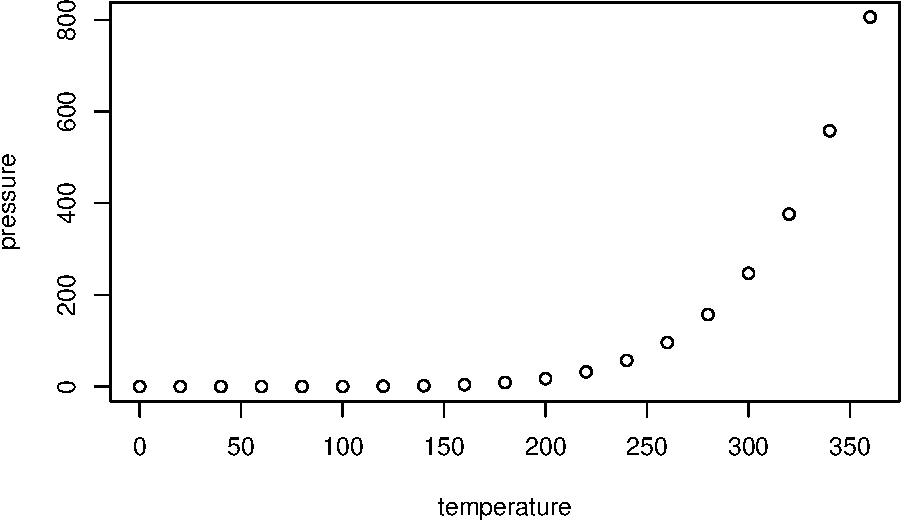
\includegraphics{test_files/figure-latex/pressure-1.pdf}

Note that the \texttt{echo\ =\ FALSE} parameter was added to the code
chunk to prevent printing of the R code that generated the plot.

\end{document}
